\appendix

\section{Theoretical Analysis: Full Derivations}
\label{app:theory_full}

\subsection{Why Sign Misattribution is the Core Mechanism}
\label{app:sign_fundamental}

The two mechanisms identified in Section~\ref{sec:dual_mechanism} operate at different layers and produce qualitatively different failures. Policy information loss (Mechanism 1) operates at the inference layer, restricting the observable context and establishing a structural performance ceiling that is constant across training. Sign misattribution (Mechanism 2) operates at the training layer, corrupting gradient directions and progressively degrading performance below this ceiling.

\textit{Proof of Proposition 1.} Define ``correct sign'' as follows: for a window containing locally beneficial actions, the correct sign of $\hat{A}_w$ is positive (reinforcement); for a window containing locally detrimental actions, the correct sign is negative (suppression). Under binary reward, the return for window $w$ is $R_w = \gamma^{(N-w)} \cdot R_{\text{episode}}$ (Equation~\ref{eq:step_return}). In a failed episode ($R_{\text{episode}} = 0$), all windows receive $R_w = 0$ regardless of their local action quality. If the group contains at least one successful rollout, the group mean $\mu > 0$, and all windows in the failed episode receive negative advantages after normalization via Equation~\ref{eq:grpo_advantage}. This includes windows where the agent took locally correct actions. Now consider a window with locally correct actions. In a successful episode (probability $p$), the window receives positive $\hat{A}_w$, which is the correct sign. In a failed episode (probability $1 - p$), the window receives negative $\hat{A}_w$ whenever $\mu > 0$, which is the wrong sign. The probability that $\mu = 0$ (all $K$ rollouts in the group failed) is $(1-p)^K$, which shrinks exponentially with $K$. As $K$ grows, nearly every failed episode produces a non-zero group mean, and the window receives the wrong sign with probability approaching $1-p$. The probability of correct sign therefore approaches $p$. \hfill$\square$

The distinction between sign error and magnitude error further clarifies why Mechanism 2 is catastrophic while Mechanism 1 is merely suboptimal. The discount factor $\gamma^{(N-w)}$ in Equation~\ref{eq:step_return} introduces magnitude decay across window positions: for an episode with $T=50$ steps and $h=2$, the first window ($w=1$) retains $\gamma^{N-1} = 0.95^{24} \approx 0.29$ of the terminal window's return. This attenuation reduces the gradient magnitude for early windows but preserves the gradient direction. A gradient with correct sign and reduced magnitude produces slow convergence, a condition recoverable through longer training. A gradient with wrong sign produces active divergence: the optimization pushes the policy away from good behaviors and toward bad ones.

\subsection{Formal Probability Analysis}
\label{app:formal_probability}

\textit{Derivation of Proposition 2.} For a window with locally correct actions, the gradient direction depends on $\text{sign}(\hat{A}_w)$, which depends on whether the episode succeeded and whether the group contains any successful rollouts. Three mutually exclusive cases arise.

\textit{Case 1: Episode succeeded} (probability $p$). The window receives $R_w = \gamma^{(N-w)} \cdot r_+ > 0$. With at least one failed rollout in the group, $R_w > \mu$ after normalization, producing $\hat{A}_w > 0$.\footnote{The edge case where all $K$ rollouts succeed (probability $p^K$) is negligible at the baseline success rates considered ($p^8 < 10^{-7}$ at $p = 12.5\%$).} The gradient reinforces the window's actions. For a window with locally correct actions, this is the correct direction.

\textit{Case 2: Episode failed, group contains at least one success} (probability $(1-p)[1 - (1-p)^{K-1}]$). The window receives $R_w = 0 < \mu$, producing $\hat{A}_w < 0$. The gradient suppresses the window's actions. For a window with locally correct actions, this is the wrong direction.

\textit{Case 3: Episode failed, entire group failed} (probability $(1-p) \cdot (1-p)^{K-1} = (1-p)^{K}$). All returns are zero, so $\mu = 0$ and $\sigma = 0$. The advantage is zero, producing no gradient update.

Summing Cases~1 and~3 yields $P(\text{correct sign or no update}) = p + (1-p)^{K}$. Since only Cases~1 and~2 produce non-zero gradients, the conditional probability follows as Equation~\ref{eq:correct_conditional}.

\label{app:nonbinary_extension}
\textit{Two calibers of credit assignment failure.} Proposition~2 and the empirical credit agreement rate (Section~\ref{sec:sign_verification}) quantify different aspects of credit assignment failure under different reward structures; both confirm that advantage sign carries insufficient information about local action quality.

\textit{Binary caliber} ($P(\text{correct} \mid \text{update}) \leq 19.1\%$). Under pure binary reward $R \in \{0, r_+\}$, the GRPO advantage $\hat{A}_w = R_w - \bar{R}_g$ has its sign entirely determined by episode outcome: all windows in a successful episode receive positive advantage, all windows in a failed episode receive negative advantage whenever the group contains at least one success. This near-deterministic sign-episode mapping, confirmed empirically at 99.6\% ($270/271$ windows; Section~\ref{sec:sign_verification}), means Proposition~2's upper bound applies directly: at most 19.1\% of non-zero gradient updates carry the correct sign.

\textit{Penalty caliber} (credit agreement $= 52.1\%$). Introducing a format penalty $r_- = -0.1$ per invalid action breaks this deterministic mapping. Within a failed episode, windows with valid actions receive $R_w = 0$ while windows with invalid actions receive $R_w = -0.1h$. This intra-episode variance shifts $\bar{R}_g$ downward, allowing some valid-action windows in failed episodes to obtain $\hat{A}_w > 0$ despite overall failure. Credit agreement rises from 19.1\% to 52.1\%, but this is marginally above random chance (Cohen's $h = 0.041$, below the 0.2 small-effect threshold), carrying negligible information about local action quality.

\textit{Complementary evidence.} The two calibers capture qualitatively different failure modes: 19.1\% reflects deterministic misattribution (advantage sign systematically tracks the wrong signal), while 52.1\% reflects near-random noise (advantage sign carries almost no local information). Both are far below the level required for policy improvement. The gap between them is itself informative: it quantifies how penalty-induced variance transforms the failure mode from systematic wrong-sign to random noise, without repairing credit assignment. A binomial test rejects $H_0{:}\, P = 0.191$ ($z = 45.9$, $p < 10^{-100}$), formally confirming that the two calibers measure different quantities.

We evaluate these expressions at the empirical baseline of our experiments. At $p = 12.5\%$ and $K = 8$: $(1-p)^K = 0.875^8 \approx 0.344$, giving $P(\text{correct or no update}) \approx 0.469$. Of the 65.6\% of cases that produce a gradient update, only $P(\text{correct} \mid \text{update}) = 0.125 / 0.656 \approx 19.1\%$ have the correct sign. As $K$ increases to 16, $(1-p)^{K} \approx 0.118$, and $P(\text{correct} \mid \text{update}) \approx 14.2\%$. In the large-$K$ limit, $P(\text{correct} \mid \text{update}) \to p$, so approximately $1 - p = 87.5\%$ of all gradient updates for locally correct windows point in the wrong direction.

\subsection{Why the Community Defaults to Step-Independent Training}
\label{app:why_defaults}

If step-independent training is structurally flawed for multi-turn agents, why has it become the default? We identify six contributing factors.

\textbf{1. Context length constraints.} Smaller language models (1B to 4B parameters) typically support context lengths of 2048 to 4096 tokens. Multi-turn episodes spanning 50 or more interaction steps easily exceed these limits. Step-independent windowing is a pragmatic response to a hardware constraint, not a deliberate algorithmic choice.

\textbf{2. Token-level training inertia.} Language model training is organized around predicting the next token over fixed-length sequences. When multi-turn RL inherits this paradigm, the natural unit of optimization becomes a fixed-length window rather than a variable-length episode. The mismatch between token-level optimization and episode-level credit assignment goes unquestioned because it aligns with existing training infrastructure.

\textbf{3. Inherited framework default.} The RAGEN framework~\citep{ragen2025} implements step-independent mode as its default configuration, not as one option among alternatives. Users inherit this choice without an explicit decision point, and default configurations propagate silently through downstream projects.

\textbf{4. Memory and compute constraints.} Episode-level training requires processing $O(T)$ tokens per sequence, incurring $O(T^2)$ attention cost with full self-attention. Step-independent training reduces this to $O(h)$ tokens and $O(h^2)$ attention cost per window. The computational savings are immediate and measurable, while the credit assignment failure is subtle and deferred until training collapse occurs.

\textbf{5. Reward shaping as apparent fix.} Dense reward shaping (per-step bonuses for intermediate goals) appears to address sparse reward problems. Our dense reward experiment (Section~\ref{sec:results_dense}) reveals a different failure mode: the agent maximizes format-level rewards (action validity rises from 60\% to 97.5\%) while task success remains at 0\%. Reward shaping does not resolve sign misattribution; it creates new optimization targets that the agent can game without solving the underlying task.

\textbf{6. Absence of negative results.} When step-independent training fails, practitioners attribute the failure to insufficient hyperparameter tuning or the inherent difficulty of sparse rewards. Without published analyses that isolate the credit assignment mechanism as the root cause, the community cannot distinguish between ``this problem is hard'' and ``this training paradigm is broken for this class of problems.''

\subsection{Connection to Classical Credit Assignment}
\label{app:classical_connection}

Our findings connect to a long line of work on temporal credit assignment in reinforcement learning.

\textbf{Temporal difference learning and eligibility traces.} Sutton's TD($\lambda$)~\citep{sutton1988td} provides a spectrum of credit assignment strategies parameterized by $\lambda \in [0,1]$. At $\lambda = 0$, credit is assigned via one-step bootstrapped returns. At $\lambda = 1$, TD($\lambda$) reduces to Monte Carlo returns. Step-independent training falls below this spectrum: windows are disconnected from each other, so temporal propagation of credit does not occur.

\textbf{Generalized Advantage Estimation.} GAE($\lambda, \gamma$)~\citep{schulman2016gae} extends TD($\lambda$) with a separate discount factor. GAE(1, 1) produces undiscounted Monte Carlo returns and is equivalent to episode-level GRPO without a critic. The key difference is that GAE uses value function subtraction as the baseline, while GRPO uses group normalization.

\textbf{REINFORCE.} Williams' REINFORCE algorithm~\citep{williams1992reinforce} computes policy gradients from complete episode returns with a learned baseline $b(s)$. Episode-level GRPO is equivalent to REINFORCE where the group mean $\mu$ replaces $b(s)$ and the group standard deviation $\sigma$ provides normalization. The algorithmic structure is not new. Our contribution is the diagnosis: the community's standard adaptation of this algorithm for multi-turn LLM agents (step-independent windowing) silently breaks the credit assignment structure that REINFORCE assumes.

\textbf{Multi-agent credit assignment analogy.} Step-independent windows can be understood through cooperative multi-agent games. Each window acts as an independent ``agent'' sharing a team reward but optimized without knowledge of other windows' actions. The sign misattribution problem parallels team reward credit assignment in cooperative multi-agent RL: when the team fails, all agents receive identical penalties regardless of individual contribution. In multi-agent RL, this is a recognized problem with known solutions such as counterfactual baselines and value decomposition methods.

\section{Hyperparameters}
\label{app:hyperparameters}

\begin{table}[h]
\centering
\caption{Shared RL training hyperparameters across all conditions.}
\label{tab:hyperparameters_app}
\begin{tabular}{lc}
\toprule
Parameter & Value \\
\midrule
Group size $K$ & 8 \\
Learning rate & $1 \times 10^{-6}$ \\
KL penalty $\beta$ & 0.01 \\
Discount $\gamma$ & 0.95 \\
Invalid action penalty & 0.1 \\
Tasks per training step & 16 \\
Training steps & 15 \\
\bottomrule
\end{tabular}
\end{table}

All 1.7B experiments were conducted on 2$\times$ NVIDIA RTX PRO 6000 GPUs. Each training run (15 steps, $K{=}8$ rollouts per task, 16 tasks per step) required approximately 6--8 GPU-hours. The 11-seed evaluation totaled ${\sim}$80 GPU-hours. The 8B experiment used 4$\times$ RTX PRO 6000 with Fully Sharded Data Parallel (FSDP), requiring ${\sim}$24 GPU-hours per run. ScienceWorld experiments used the same 2-GPU setup as the 1.7B ALFWorld runs.

\paragraph{SFT baseline.} The base policy was fine-tuned on 2{,}546 expert demonstrations from the ALFWorld training split following the protocol of RAGEN~\citep{ragen2025}, using learning rate $5 \times 10^{-6}$, batch size~16, and 2 epochs.

\section{Cross-Scale and Cross-Environment Results}
\label{app:8b_results}

\begin{figure*}[t]
\centering
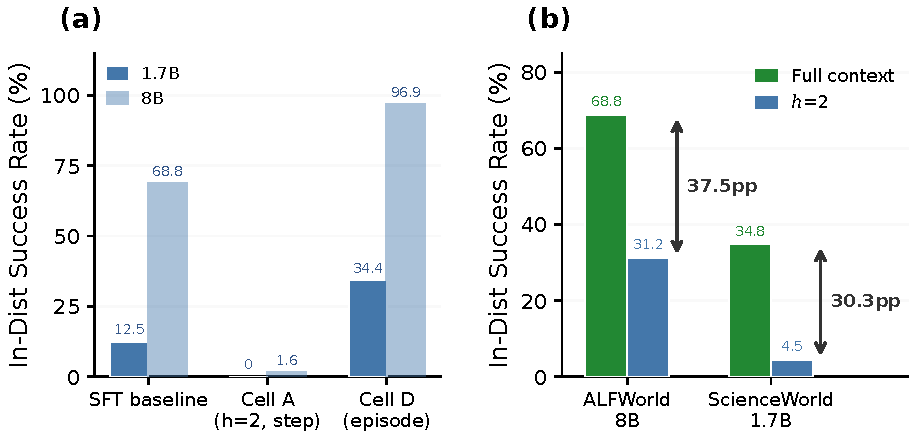
\includegraphics[width=\textwidth]{fig_cross_scale.pdf}
\caption{(a)~Cross-scale verification (single seed): both collapse (Cell~A) and fix (Cell~D) are observed from 1.7B to 8B. The episode-level fix appears more effective at 8B (96.9\% vs.\ 34.4\% in-distribution). (b)~Information loss (M1) quantification (single seed each): restricting context to $h{=}2$ drops SFT performance by 37.5pp at 8B ALFWorld and 30.3pp on ScienceWorld.}
\label{fig:cross_scale}
\end{figure*}

\begin{table}[h]
\centering
\caption{8B results on ALFWorld. SFT and $h{=}2$ use decoding temperature $\tau{=}0$; RL uses $\tau{=}0.4$. Cell~A: step~2 (post-collapse). Cell~D: step~10. Single seed. The primary comparison is Cell~A collapse (0\%) vs Cell~D success, which is independent of decoding temperature.}
\label{tab:8b_results}
\small
\begin{tabular}{@{}lcc@{}}
\toprule
\textbf{Method} & \textbf{In-Dist (\%)} & \textbf{OOD (\%)} \\
\midrule
SFT baseline & 68.75 & 80.60 \\
SFT $h{=}2$ & 31.25 & --- \\
Cell A: step-indep.\ ($h{=}2$) & 28.1 $\to$ 1.6 & --- \\
Cell D: episode-level & \textbf{96.88} & \textbf{90.30} \\
\bottomrule
\end{tabular}
\end{table}

\section{Additional Conditions}
\label{app:additional}

All conditions use single seeds unless noted.

\paragraph{Dense reward.} Step-independent $h{=}2$ with $+0.15$ per valid action. Action validity rises from 60\% to 97.5\% while task success remains 0\%; the agent games format-level rewards without solving tasks (Figure~\ref{fig:additional_conditions}b).
\label{sec:results_dense}

\paragraph{REINFORCE++.} Episode-level with per-token running-mean baseline (no critic). REINFORCE++ matches the SFT baseline (12.50\%) without improvement, suggesting that per-token advantage normalization alone does not help when the per-token baseline lacks a learned value function. This is a preliminary comparison over 15 training steps; we cannot conclude that REINFORCE++ would fail with longer training or different hyperparameters. The result suggests that naive algorithm substitution without addressing M1/M2 is insufficient, but a definitive comparison would require matched compute budgets and hyperparameter sweeps. OOD evaluation was not conducted as REINFORCE++ showed no improvement over SFT on the in-distribution set.

\begin{table}[h]
\centering
\caption{Additional baselines on ALFWorld (1.7B). Neither method improves over the SFT baseline on in-distribution tasks.}
\label{tab:additional_baselines}
\small
\begin{tabular}{@{}lccc@{}}
\toprule
\textbf{Method} & \textbf{Best Step} & \textbf{In-Dist (\%)} & \textbf{OOD (\%)} \\
\midrule
SFT baseline & --- & 12.50 & 6.72 \\
Dense reward ($h{=}2$) & 5 & 0 & 0 \\
REINFORCE++ & 5 & 12.50 & --- \\
\bottomrule
\end{tabular}
\end{table}

\paragraph{Discount factor sweep.} $\gamma \in \{0.50, 0.80, 0.95, 1.00\}$ at $h{=}5$. All four collapse to 0\% within 5 steps, including $\gamma{=}1.0$ where no magnitude decay exists. This confirms sign misattribution, not discounting, is the operative mechanism (Figure~\ref{fig:additional_conditions}a).

\begin{figure*}[t]
\centering
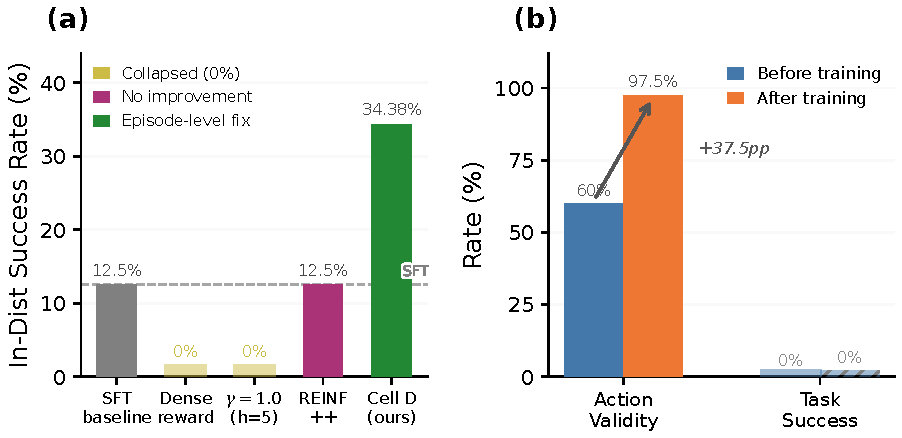
\includegraphics[width=\textwidth]{fig_additional_conditions.pdf}
\caption{(a)~Standard remedies for step-independent training: dense reward shaping and discount factor $\gamma{=}1.0$ both collapse to 0\%; REINFORCE++ matches the SFT baseline without improvement. Only episode-level training (Cell~D) exceeds baseline. (b)~Dense reward gaming: action validity rises from 60\% to 97.5\% while task success remains 0\%; the agent maximizes format-level rewards without solving tasks.}
\label{fig:additional_conditions}
\end{figure*}

\paragraph{Cell~C attempt.}
\label{app:cell_c}
Cell~C (full observation + step-level advantage) would isolate M2 without M1. We attempted this configuration across six training runs with varying hyperparameters (KL penalty $\beta \in \{0.001, 0.01, 0.04\}$, learning rate $\in \{5{\times}10^{-7}, 10^{-6}\}$). All runs terminated due to training instability: KL divergence spiked above 10.0 within 2--3 steps, triggering NaN losses. We attribute this to the combination of full-length sequences ($>$4096 tokens) with step-level advantage normalization, which produces extreme advantage magnitudes at early window positions. Cell~C remains an important gap in the partial factorial; addressing it likely requires architectural changes (e.g., gradient clipping per window position) beyond the scope of this diagnostic study.


\section{Method Selection Guide}
\label{app:method_selection}

The M1/M2 diagnostic framework guides practitioners toward the appropriate fix without exhaustive ablation. If only M2 is active (sign misattribution with sufficient observation context, e.g., $h$ large enough to preserve task-relevant information), per-step credit methods (Turn-PPO~\citep{turnppo2025}, HCAPO~\citep{hcapo2026}, GiGPO~\citep{feng2025gigpo}) directly address the failure mode. If only M1 is active (information loss without sign corruption), increasing $h$ or switching to full-context encoding suffices. When both co-occur (the typical default configuration), episode-level methods address both simultaneously. Finer-grained credit methods should be applied only after establishing an episode-level baseline, as they assume correct gradient direction.

\section{Response Length During Training}
\label{app:response_length}

\begin{figure}[h]
\centering
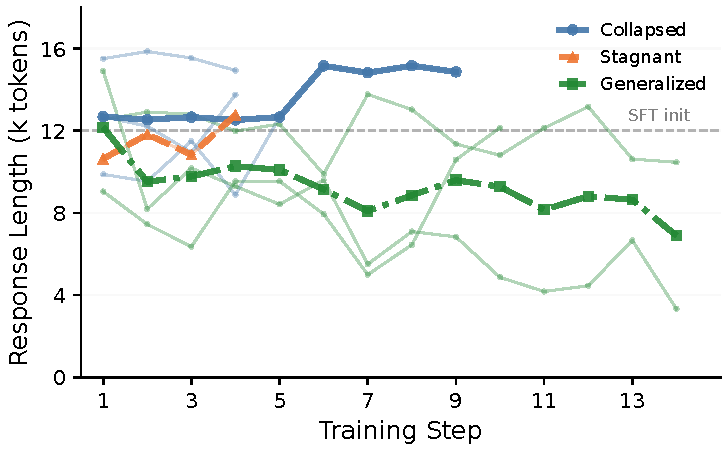
\includegraphics[width=\columnwidth]{fig_response_length.pdf}
\caption{Response length over training for 7 seeds under episode-level GRPO. Collapsed seeds (red) exhibit length inflation to 14{,}000--16{,}000 tokens. Generalized seeds (green) maintain or reduce response length. Stagnant seed (orange, seed100) remains near the SFT initialization.}
\label{fig:response_length}
\end{figure}

\section{Unified Step-5 Evaluation}
\label{app:step5_unified}

To guard against cherry-picking of checkpoints, Table~\ref{tab:step5_unified} reports all 11 seeds at a fixed evaluation point (training step~5). OOD results are included only for seeds with checkpoints evaluated under our 134-task OOD evaluation protocol (Section~\ref{sec:setup}); remaining checkpoints were unavailable for post-hoc OOD evaluation.

\begin{table}[h]
\centering
\caption{Episode-level GRPO: all 11 seeds at training step~5 (134 OOD tasks, 32 ID tasks, $\tau{=}0.4$). SFT baseline: 12.5\% ID, 6.72\% OOD. OOD results marked ``---'' indicate checkpoints unavailable for post-hoc evaluation on the 134-task OOD set. ID results marked ``---'' indicate step-5 validation metrics not recorded in training logs.}
\label{tab:step5_unified}
\small
\setlength{\tabcolsep}{4pt}
\begin{tabular}{@{}lcccc@{}}
\toprule
\textbf{Seed} & \textbf{Cat.} & \textbf{ID} & \textbf{OOD} & \textbf{vs SFT} \\
\midrule
seed2048 & C & --- & 8.21 & NS \\
seed8 & C & 28.13 & 11.94 & NS \\
seed42 & C & 9.38 & 12.69 & NS \\
\midrule
seed200 & S & --- & 10.45 & NS \\
seed300 & S & 25.00 & 10.45 & NS \\
seed100 & S & 31.25 & 11.19 & NS \\
seed2 & S & --- & --- & --- \\
\midrule
seed1 & G$^\dagger$ & --- & 23.88 & $p{<}0.001$ \\
seed4 & G & --- & --- & --- \\
seed5 & G & --- & --- & --- \\
seed6 & G & 21.88$^\ddagger$ & --- & --- \\
\bottomrule
\end{tabular}
\begin{flushleft}
\small $^\dagger$ RAGEN built-in eval; checkpoint unavailable for re-evaluation. \\
\small $^\ddagger$ Registry value 21.9\% (7/32); rounded to 21.88\% for consistency with 32-task denominator.
\end{flushleft}
\end{table}

\section{Evaluation Variance Analysis}
\label{app:eval_variance}

To quantify evaluation noise at $\tau{=}0.4$, we evaluate a single checkpoint (seed200, step~5) three times independently on the 134-task OOD set with different random seeds.

\begin{table}[h]
\centering
\caption{Evaluation variance for a single checkpoint (seed200 step~5, 134 OOD tasks, $\tau{=}0.4$). Three independent runs yield std$=$1.29pp, an order of magnitude smaller than the inter-seed performance range in Table~\ref{tab:seed_variability} (8.2\%--30.6\%).}
\label{tab:eval_variance}
\small
\setlength{\tabcolsep}{3pt}
\begin{tabular}{@{}lcccc@{}}
\toprule
\textbf{Checkpoint} & \textbf{Runs} & \textbf{OOD (\%)} & \textbf{Std} & \textbf{Range} \\
\midrule
seed200 step~5 & 3 & 11.94 & 1.29 & 2.24 \\
\bottomrule
\end{tabular}
\end{table}

The small standard deviation (1.29pp) confirms that the large inter-seed differences observed in Table~\ref{tab:seed_variability}, ranging from 8.2\% (collapsed) to 30.6\% (generalized), reflect genuine training dynamics rather than evaluation noise. We note that this variance estimate is based on a stagnant seed (seed200); generalized seeds with higher success rates may exhibit different variance profiles due to the non-linear relationship between success rate and binomial variance.

The classification threshold between stagnant and generalized seeds is based on Fisher's exact test at $p < 0.01$ vs.\ the SFT baseline; shifting to $p < 0.05$ would reclassify seed2 (the marginal case at $p = 0.03$) as generalized, changing the generalization rate from 36\% to 45\%.

\paragraph{Training efficiency.} Episode-level training processes the same total tokens as step-independent training but in fewer, longer sequences. On our hardware (2$\times$ RTX PRO 6000, 1.7B model), step-independent training ($h{=}2$) completes 15 steps in approximately 10--12 hours; episode-level training takes comparable wall-clock time as the increased sequence length is offset by fewer padding tokens.

\section{Early Training Signal Analysis}
\label{app:early_signal}

We investigated whether early training signals (steps 1--3) can predict seed-level generalization outcomes. We analyze 12 seeds grouped into three outcome categories following the definitions in Section~\ref{sec:seed_variability}: Generalized ($n{=}4$), Stagnant ($n{=}4$), and Collapsed ($n{=}4$, including seed7, which received a subsequent KL penalty intervention and is excluded from Table~\ref{tab:seed_variability}; its pre-intervention training trajectory is used here). No standard training metric (reward, KL divergence, entropy, gradient norm, response length, or train success rate) showed statistically significant between-group differences in the first three training steps (all Welch $t$-test $p > 0.2$, $n = 4$ per group). Two of the four Collapsed seeds (seed7, seed8) exhibited among the \textit{highest} early rewards and train success rates, with their collapse manifesting only after step~5 through response length inflation or reward degradation.

The strongest candidate predictor was the mutual information diversity estimate at step~1, which showed a large effect size (Cohen's $d = 1.11$) favoring Generalized over Collapsed seeds and a trending correlation with final OOD performance (Spearman $\rho = 0.43$, $p = 0.19$), but remained non-significant with the available sample size ($n = 4$ per group). These results suggest that seed-dependent outcomes are governed by mechanisms not captured by standard early training diagnostics, and that early stopping or seed selection based on initial step metrics would be unreliable.

\section{Use of AI Assistance}
We used Claude for coding, code drafting, debugging, and language polishing.
